%\addbibresource{/home/jorgsk/phdproject/bibtex/jorgsk.bib}

This chapter concerns the investigation of polyadenylation sites from RNA-seq
data. I developed a software called Utail (detailed in the Appendix on page
\pageref{utail}) and ran it on RNA-seq data to characterize polyadenylation
sites in 12 human cell lines. Parts of the analysis was published as part of
the ENCODE project by Djabeli et al.\ in the paper ``Transcription landscape of
human cells'', which is attached on page \pageref{landscape} in the Appendix.
We begin this chapter by briefly explaining what the ENCODE project is about.
Then I summarize the findings in the Djabeli et al. and my contribution to it.
Finally I cover the findings from my investigation that were not included in
the paper.

\section{The ENCODE pilot project}
The complete human genome was published in 2003 (augmenting the working draft
that was published in 2001). To find out what could be learned from the newly
available genome, the ENCODE (\textbf{Enc}yclopedia \textbf{O}f \textbf{D}NA
\textbf{E}lements) pilot project was launched to investigate in detail 1\% of
the human genome through a collaboration of research labs all over the world.
With the then prevalent genome-wide technologies, which included among others
microarrays, CAGE, and ChIP-Chip, combined with bioinformatic analysis, the
outcome of the ENCODE pilot was a wealth of data that confirmed previous
tentative genome-wide findings, added new knowledge, and was used to improve
the annotation the human genome. The outcome was published in a summary paper
in Nature \cite{birney_identification_2007} as well as in 28 companion papers
in a special edition of Genome Research. The data generated by ENCODE is freely
available from http://genome.ucsc.edu/ENCODE/ including important metadata
about how the experiments were performed.

\section{The ENCODE follow-up project}
The ENCODE pilot was deemed a success and led to a follow-up project that would
cover 100\% of the genome. This was made possible by the then-emerging
next-generation DNA sequencing technology which had considerably lowered the
cost of sequencing while also increasing the throughput. The technologies from
the ENCODE pilot were mostly replaced with the next-generation version:
microarrays were generally substituted for RNA-seq, CAGE could use next-gen
sequencers instead of Sanger sequencing, and ChIP-Chip was replaced by
ChIP-seq. As of autumn-2012 most of the follow-up ENCODE papers have been
published \cite{consortium_integrated_2012}.

\section{Summary of the paper}
The paper by Djabeli et al.\ focuses in on the RNA-seq data from ENCODE in
order to characterize the transcriptome of human cell lines. They found that
the cumulative RNA coverage for 15 human cell lines is 62\% for processed
transcripts and 75\% for primary transcripts (e.g. pre-mRNA). In other words,
three quarters of the human genome is transcribed. However, the average
transcript coverage for each cell line was 22\% and 39\% for processed and
primary transcripts. This tells us that while most of the genome is capable of
being transcribed, each cell line will express little more than a quarter of
it. Using the Cufflinks software, which assembles a transcriptome from RNA-seq
data \cite{trapnell_transcript_2010}, they discovered 45\% more transcripts
than are currently annotated, with most of the newly identified transcripts
coming from intergenic regions. As a result, the median length of intergenic
regions decreased from around 14.000 bp to 4.000 bp, showing that the human
genome is not as "barren" as was once thought. The study identified around
22.000 new RNA splice sites, demonstrating the flexibility of the human genome
whereby each gene may express multiple RNA isoforms. Many genes were found to
express up to 12 alternative isoforms, although more than 30 \% of gene
expression can be attributed to one dominant isoform. It was found that three
quarters of protein coding genes have at least two dominant isoforms. This
shows that while alternative isoform usage is ubiquitous, in general a few
dominating isoforms exist for each gene. Additionally, they discovered many new
long noncoding RNAs (lncRNA). These RNAs appear similar to mRNA and undergo
processing, but do not code for protein. An over-all conclusion about
expression levels is that protein coding transcripts are highly expressed,
while non-coding transcripts like lncRNA are generally lowly expressed, down to
less than one transcript estimated per cell. Using PET-data, they discovered
roughly 128.000 transcription start sites, of which around 30.000 were novel.
They also discovered around 129.000 cleavage and polyadenylation sites inside
annotated transcripts, 80\% of which were not previously annotated. The last
finding suggest that transcription start sites are generally better annotated
than transcript end sites.

\section{My contribution}
My contribution to the paper was the identification of the 129.000
polyadenylation sites in annotated regions.

\section{Results}
When investigating the polyadenylation sites for the Djabeli et al.\ paper,
many results came up that were not included in the paper due to limitations in
space. Here follow those results.

\subsection{Dataset}
The analysis of RNA-seq data has become a successful approach for studying
genome-wide patterns of polyadenylation \cite{shepard_complex_2011,
ozsolak_comprehensive_2010}. However, the dataset used in this analysis is
different from most RNA-seq libraries that have been used to study
polyadenylation. Prior to sequencing, cells have been separated in to
cytoplasmic and nuclear fractions. Data is therefore available for whole cell,
cytoplasmic, an nuclear RNA. Further, all compartments were further separated
into poly(A)+ and poly(A)- fractions before sequencing. As previously
mentioned, the poly(A)+ fraction of an RNA sample contains all the RNA that is
captured by a poly(T) primer. This includes all RNA with a poly(A) tail of more
than 20 nucleotides (the length of the poly(T) primer).

\subsection{Total number of polyadenylation sites}
By merging all polyadenylation sites from all datasets (see Table
\ref{tab:datasets}), we identified a total of 163.537 polyadenylation sites in
the genome for the poly(A)+ fraction, around 129.000 of which were in annotated
regions. 94040 or 58\% of these sites were found with a downstream PAS (within
40 nt) and 33054 or 20\% were previously annotated in GENCODE or in polyAdb
\cite{lee_polya_db_2007}. In addition, we found 57.031 polyadenylation sites
for the poly(A)- fraction, many of which overlapped the polyadenylation sites
in the poly(A)+ fraction.

Figure \ref{fig:saturation} shows how the number of polyadenylation sites
saturates as the number of included datasets increases. The saturation is
sharper both for polyadenylation sites which we found to have a downstream
PAS and sites supported by PET data. The saturation of polyadenylation sites is
sharper for the poly(A)- fraction (Figure \ref{fig:saturation}B), and fewer of
the poly(A)- sites are associated with PAS or PET.

\subsection{Distribution of polyadenylation sites across the genome}
As expected, we found that most of the polyadenylation sites were in the 3\ppp
UTR exonic regions, but we located many polyadenylation sites in the intergenic
and intronic regions as well (Figure \ref{fig:sidebars}). In the poly(A)+
fraction, there is more intronic polyadenylation sites in the nucleus than in the
cytoplasm. This was to a certain degree expected since there is much more
intronic RNA in the nucleus compared to the cytoplasm. However, introns do
naturally exist in the cytoplasm. Some are included as part of the final mRNA
(called intron inclusion), and some are included if an intron contains an
active poly(A) site \cite{tian_widespread_2007}. The number of polyadenylation
sites in the other genomic regions, such as the 5\ppp UTR and 3\ppp UTR
intronic regions, was low and is not shown in Figure \ref{fig:sidebars}.

The evidence for polyadenylated RNA in the poly(A)- fraction (Figure
\ref{fig:sidebars}B) was unexpected, since the poly(A)- fraction is by design
not supposed to contain RNA with poly(A) tails. We propose that the
polyadenylated RNA in the poly(A)- fraction have three possible sources (shown
in Figure \ref{fig:S123}). The first source (S1) is purely technical: normal
poly(A)+ mRNA with full length poly(A) tails may not get adsorbed during the
poly(A)+ filtration step and therefore end up in the poly(A)- fraction. Source
two (S2) and source three (S3) are on the other hand of biological origin. S2
is RNA with poly(A) tails that are shorter than 20nt, which is the threshold
length of poly(A) tails that are captured by the poly(A)+ filtration step. One
type of S2 RNA are mRNA which have had their polyA tails degraded to below 20
nucleotides, which happens during mRNA degradation, at the time of sampling.
Another type of S2 RNA are mRNA that were actively undergoing polyadenylation
at the time of sampling and did not reach a poly(A) tail length of more than 20
nucleotides. Source three (S3) on the other hand is distinct from S1 and S2. We
propose that S3 consists of RNA with the short, degradation-related transient
poly(A) tails that have been identified in the nucleus of mammalian cells
\cite{lemay_nuclear_2010}.  These RNA may be aberrant rRNA
\cite{shcherbik_polyadenylation_2010}, aberrant pre-mRNA
\cite{west_adenylation_2006}, or possibly intronic RNA undergoing degradation
\cite{schmidt_polyadenylation_2010}.

\begin{figure}[hb]
	\begin{center}
		\includegraphics[scale=0.5]{illustrations/S1S2S3.pdf}
	\end{center}
	\caption{Different proposed origins of polyadenylation signals in poly(A)-.
	\textbf{S1} RNA is a result of random error in the technical separation of poly(A)+
	and poly(A)- RNA. \textbf{S2} RNA is the result of polyadenylated mRNA which have a
	short poly(A) tail at the moment of sampling, either due to early
	polyadenylation in the nucleus (upper) or degradation in the cytoplasm
	(lower). \textbf{S3} RNA are proposed to be RNA undergoing
	poly(A)-dependent degradation in the nucleus.}
	\label{fig:S123}
\end{figure}

\subsection{Isolating polyadenylation sites unique to the poly(A)- and poly(A)+
fractions}
We wanted to separate the S3 from the S1 and S2 polyadenylation sites in the dataset.
We did this by assuming that many of the S1 and S2 sites are likely to be
present in both the poly(A)- and the poly(A)+ fractions, since these sites by
definition are normal polyadenylated RNA that have ended up in the poly(A)-
fraction. Therefore, we filtered out all the polyadenylation sites that were common to
the poly(A)+ and poly(A)- fraction and removed these from both fractions. After
removing the polyadenylation sites common to poly(A)- and poly(A)+, a difference
emerged in the now ``pure'' fractions. As can be seen in in Figure
\ref{fig:sidebars_intersect}, almost no polyadenylation sites were found in the pure
poly(A)- fraction of the cytoplasm. The pure nuclear poly(A)- fraction has
fewer polyadenylation sites in the 3\ppp UTR exonic region compared to the
original poly(A)- fraction, while the number of sites in the intergenic and
intronic regions did not change much.

\begin{figure}[hb]
	\begin{center}
		\includegraphics[scale=0.3]{figures/polyadenylation/fixed_Saturation_plot_2+.pdf}
	\end{center}
	\caption{The number of identified polyadenylation sites increases and
	slowly saturates as more datasets are included. \textbf{A}: poly(A)+
	RNA. \textbf{B}: poly(A)- RNA.}
	\label{fig:saturation}
\end{figure}

\begin{figure}[hb]
	\begin{center}
		\includegraphics[scale=0.3]{figures/polyadenylation/fixed_intersected_sidebars_pA_2+.pdf}
	\end{center}
	\caption{Number of polyadenylation sites across genomic regions for RNA
	unique and common to poly(A)+ and poly(A)- RNA. The left and right columns
	show the number of polyadenylation sites after removing the sites common to
	the poly(A)+ and poly(A)- fractions. The middle column shows the sites that
	overlapped. Row one, two, and three show polyadenylation sites in the whole
	cell, cytoplasm, and nucleus, respectively. The blue line indicates the
	fraction of sites which had a PAS within 40 basepairs downstream. The green
	line shows the sites found within 50 nucleotides of a PET signal.}
	\label{fig:sidebars_intersect}
\end{figure}

\begin{figure}[hb]
	\begin{center}
		\includegraphics[scale=0.35]{figures/polyadenylation/fixed_Sidebars_pA_2+.pdf}
	\end{center}
	\caption{Polyadenylation across genomic regions for the poly(A)+ and poly(A)-
	fractions. See Figure \ref{fig:sidebars_intersect} for further description.}
	\label{fig:sidebars}
\end{figure}

\section{Discussion}
Polyadenylation is a post-transcriptional modification of RNA with two opposite
regulatory functions. The poly(A) tail confers stability when it is is added as
part of mRNA processing. Conversely, the poly(A) tail signals for degradation
when used in bacteria and as recently discovered for some RNA species in
eukaryotes \cite{shcherbik_polyadenylation_2010}.

Here we have investigated sites of polyadenylation in the transcriptome in an
RNA-seq library that contains data from RNA both in the whole cell and in the
nuclear and cytoplasmic compartments. Further, the RNA in the library was
separated in the poly(A)+ and poly(A)- fractions.

The discovery of polyadenylation sites saturated slowly for all sites, but
sharply for sites associated with a PAS or supported by PET (Figure
\ref{fig:saturation}). We consider polyadenylation sites with a downstream PAS
to be more likely to be true positives. Thus, the different saturation curve
for non-PAS and PAS-associated polyadenylation sites indicates that the number
of false positives increases when a large number of datasets are included.

We found many polyadenylation sites in intergenic regions (Figure
\ref{fig:sidebars}), which are regions of the genome that do not contain
annotated genes. These sites may represent either unannotated 3\ppp UTR
ends from known genes or cleavage and polyadenylation sites of novel
transcripts.

In general, we see that the pattern of polyadenylation in the whole cell
extracts looks like the sum of the polyadenylation sites in the nuclear and
cytoplasmic extracts (Figure \ref{fig:sidebars}). This is as expected; the
nucleus and the cytoplasm make up the whole cell. However, it shows the power
of studying the individual compartments instead of just the whole cell. All
studies of polyadenylation to date have used whole cell extracts. These studies
would only see the top row in Figure \ref{fig:sidebars}. That the intronic
polyadenylation sites come mainly from the nucleus would be difficult to infer
without compartmentalized RNA-seq data.

Before removing ther polyadenylation sits common to the poly(A)+ and poly(A)-
RNAs, there were few polyadenylation sites in the cytoplasmic poly(A)- RNA,
and most of then in 3\ppp UTR exonic regions (Figure \ref{fig:sidebars}D).
However, after removing the polyadenylation sites common to the poly(A)+ and
poly(A)- RNAs, it became clear that practically all the polyadenylation sites in
the cytoplasmic poly(A)- RNA were in common with the poly(A)+ RNA
(compare Figure \ref{fig:sidebars_intersect}E and
\ref{fig:sidebars_intersect}F). The pure cytoplasmic poly(A)- RNA is
therefore practically void of polyadenylation sites. This indicates that there
are very few RNA with short poly(A) tails in the cytoplasm. We propose that the
signals common to the poly(A)+ and poly(A)- RNAs in the cytoplasm
originate from normal polyadenylated mRNA that had their poly(A) tails reduced
to less than 20 nt because they were undergoing degradation (see the lower S2
RNA in Figure \ref{fig:S123}).

The low number of unique polyadenylation sites in the pure poly(A)- RNA of the
cytoplasm (Figure \ref{fig:sidebars_intersect}F) may be an indication that the
number of false positives in the study is not high. Presumably false positives
are not biased toward any compartment or any of the poly(A)- or poly(A)+
fractions, so the polyadenylation sites in the poly(A)- RNA in the cytoplasm
may be an indication of the number of false positives in the study. 

The nuclear poly(A)- RNA was found to be enriched in polyadenylation sites
compared to the cytoplasic poly(A)- RNA (Figure \ref{fig:sidebars}F compared to
Figure \ref{fig:sidebars}D). As was found for cytoplasmic RNA, removing the
common sites with the poly(A)+ RNA revealed that most polyadenylation sites in
3\ppp UTR of the nuclear poly(A)- RNA were common with the poly(A)+ RNA (Figure
\ref{fig:sidebars_intersect}H). We propose that the polyadenylation sites in the 3\ppp
UTR common to the nuclear poly(A)+ and poly(A)- RNA represent mRNA undergoing
polyadenylation (see the upper S2 RNA in Figure \ref{fig:S123}).

However, unlike for the cytoplasmic RNA, there is after separation still an
enrichment of polyadenylation sites in the intergenic and intronic regions of
the poly(A)- RNA. This enrichment could be partially expected since since
introns comprise a much larger part of nuclear RNA than cytoplasmic RNA, simply
because human pre-mRNA sequences contain over 20 times more intronic than
exonic sequence \cite{venter_sequence_2001}. However, all intronic sites are
not likely to be false positives; and judging from the cytoplasmic pure
poly(A)- fraction (Figure \ref{fig:sidebars_intersect}F) the number of false
positives in the study may be low. We propose that the general enrichment in
the poly(A)- sites in the nuclear fraction compared to the cytoplasm may be due
to degradation-related transient polyadenylation that occurs in the nucleus of
mammalian cells \cite{lemay_nuclear_2010} (see S3 RNA in Figure \ref{fig:S123}.
The polyadenylated RNA in the nuclear intergenic region may stem from
degradation of spurious transcripts as found in yeast
\cite{wyers_cryptic_2005}. The polyadenylation sites in the intronic region may
stem from a yet-to-be discovered polyadenylation-mediated degradation mechanism
for introns, as has been postulated \cite{schmidt_polyadenylation_2010}.

\subsection{Summary}
In summary, by studying polyadenylation in six dimensions (whole cell,
cytoplasm, and nucleus in the poly(A)+ and poly(A)- fractions) compared to
normally just one (whole cell, poly(A)+), we have made observations that would
otherwise not be possible to make. First of all, the polyadenylation sites in
whole cell RNA were shown to be the sum of polyadenylation sites the nuclear
and the cytoplasmic RNA, which verifies the integrety of the datsets. Second,
by separating the polyadenylation sites common to poly(A)+ and poly(A)- RNA, we
were able to potentially identify between polyadenylation signals from mRNA
undergoing degradation in the cytoplasm and mRNA undergoing polyadenylation in
the nucleus. Further, we identified an enrichment in intronic and intergenic
polyadenylation sites in the poly(A)- RNA in the nucleus which is not present
in the cytoplasm. These polyadenylation sites may be traces of the newly
discovered polyadenylation-mediated degradation mechanism in the nucleus of
eukaryotic cells.  

\section{Materials and Methods}
\subsection{Methods}
The full description of the methods we used is found on page \pageref{utail} in
the Appendix as part of the description of the pipeline we developed for
analysing poly(A) sites from RNA-seq data. Briefly, the method involves
identifying poly(A) sites by trimming poly(A/T) stretches of unmappable reads,
remapping the reads after trimming, and clustering the 3\ppp ends of the mapped
reads are within 20 nucleotides of each other, since this is close to the
maximal range of the stochastic effect of choice of 3\ppp cleavage site
\cite{tian_large-scale_2005}. After clustering we searched the genomic sequence
40 nucleotides downstream the polyadenylation site for one of the
polyadenylation signals (PAS). Finally we intersected the polyadenylation sites
with the 3\ppp PET sites (see below) to see which overlapped. To avoid false
positives, we checked the genomic sequence for poly(A) tracts and discarded
putative poly(A) reads that landed at genomic locations that were poly(A) rich.
Further we filtered out poly(A) reads that mapped to intron-exon junctions,
since several false positives were found at these locations.

\subsection{The dataset}
The datasets used in this study are available from
http://hgdownload-test.cse.ucsc.edu/goldenPath/hg19/encodeDCC/wgEncodeCshlLongRnaSeq/

The data was generated from RNA-seq experiments from 12 human cell lines. Six
of the cell lines have RNA-seq data from whole cell extracts and the remaining
six cell lines have RNA-seq data from cytoplasmic and nuclear extracts in
addition to whole cell extracts. Each cell line is further available in both
the poly(A)+ and poly(A)- fractions of the RNA pool. Table \ref{tab:Datasets}
shows the cell lines and compartments used and the number of replicates. In
total, 23 datasets were from whole cell extracts, 11 from cytoplasmic extracts,
and 12 from nuclear extracts. This brings the total to 92 RNA-seq datasets. The
datasets contains only RNA-seq from long RNA, defined as RNA over 200
nucleotides in length. Each dataset has been generated with Illumina
paired-ended sequencing with a read-length of 76 basepairs and contains between
150 and 250 million reads.

\begin{table}[hb]
	\centering
	\begin{tabular}{cccc}
	  Cell line & Whole Cell & Cytoplasm & Nucleus \\
	  \midrule
	  GM12878 & 2 & 2 & 2 \\
	  K562 & 2 & 2 & 2 \\
	  HeLa-S3 & 2 & 2 & 2 \\
	  HUVEC & 2 & 2 & 2 \\
	  HEPG2 & 2 & 2 & 2 \\
	  H1Hesc & 1 & 1 & 1 \\
	  Nhek & 2 & 0 & 1 \\
	  MCF7 & 2 & 0 & 0 \\
	  AG04450 & 2 & 0 & 0 \\
	  HSMM & 2 & 0 & 0 \\
	  NHLF & 2 & 0 & 0 \\
	  A549 & 2 & 0 & 0 \\
	\end{tabular}
	\caption{Number of replicates of the compartmentalzied RNA-seq data from 12
	different cell lines from the ENCODE consortium.}
	\label{tab:Datasets}
\end{table}

\subsection{The short RNA mapper}
The short read mapper used in this work is the GEM mapper
\cite{ribeca_gem_2010}. The GEM mapper is production ready but currently still
under development.

\subsection{The PET data}
Paired End diTag (PET) sequence is a technique that is specific for locating
the 3\ppp end of transcripts. This technique adds two tags to the 3\ppp end and the
5\ppp end of an RNA. Those tags then join with each other, forming a circular
RNA. Subsequently, the sequences close to the two tags (less than 30 nt) are
sequenced. Thereby, one obtains the sequence information about both the
transcription start site and the transcript termination site of the RNA. We
have used PET data which is available from
http://hgdownload.cse.ucsc.edu/goldenPath/hg19/encodeDCC/wgEncodeGisRnaPet/ to
compare with the polyadenylation sites we discovered. We used a threshold of 10
PET reads to accept a site as transcript termination site.
